\subsection{Convenience}
Como mencionamos anteriormente, nuestro objetivo es que el usuario tenga un acceso a los datos directos sin tener que lidiar con ninguno
de los procesos tecnicos que conlleva el implementar un sistema. Los puntos que deberemos cubrir para alcanzar este objetivo son:\\
\textbf{Infraestructura}. Recoleccion de datos, procesado, almacenamiento y visualizacion. Por ejemplo, en la mayoria de los casos, los datos son 
publicados periodicamente, pero el conjunto de datos publicados solo contien las muestras mas recientes, por lo que no hay manera de obtener 
un historico de los datos si no son recolectados, procesados y almacenados periodicamente. \\
\textbf{Automatizacion}. Como comentabamos en el punto anterior, esta tareas son repetitivas y ademas tienden a ser procesos arduos, por lo que sera
necesario automatizarlo, de otra forma el esfuerzo requerido por el usuario para extraer la informacion no le compensara. \\
\textbf{Disponibilidad} Para ofrecer los datos a los usuarios de una manera directa, es recomendable utilizar una plataforma a la que el usuario
este familiarizado. Por ejemplo, es mas factible que el usuario se sienta mas atraido a acceder a los datos si no requiere
ninguna instalacion en sus dispositivos.\\

\subsubsection{How to solve it} 
Tendremos que proporcionar toda la infraestructura mencionada para poder realizar todos los pasos para completar el camino de la obtencion de los
datos en crudo hasta ofrecerselos al usuario de una manera accesible, relevante e irresistible.
Intentaremos liberar al usuario de acciones repetitivas, automatizaremos todos los procesos posibles, para ofrecer al usuario la informacion lo mas
directamente posible.
Deberemos ofrecer la informacion mediante una plataforma con que el usuario este familiarizado, hoy en dia el uso de pagina webs o aplicaciones moviles es muy comun.
Es recomendable ofrecer toda la informacion posible sin necesidad de hacer que el usuario realize acciones complicadas y no requiera de ningun software o hardware adicional.
Deberemos velar por la seguridad, por lo que la plataforma debe ser segura.

\subsubsection{How we solve it. Aire Guru} 
El conjunto de datos de la calidad del aire de Malaga se actualiza cada hora, Aire Guru automatiza el proceso de recoleccion de los 
datos mediante un trabajo CRON que ejecuta un script implementado en JavaScript periodicamente. Este lee los datos de la url, los procesa,
limpia y almacena en una base de datos MongoDB. Es decir, implementa toda la estructura necesaria.

Gracias a esta infraestructura el usuario es capaz de visualizar la evolucion de los contaminantes desde el 2018. Ademas puede ver la exposicion
personal a estos contaminante durante el mismo periodo de tiempo.

Ademas, con la automatizacion de procesos, el usuario es capaz de visualizar la polucion a tiempo de real de la ciudad de Malaga y concretamente en el punto
en el que se encuentra.\\

\begin{figure}[ht]
    \centering
    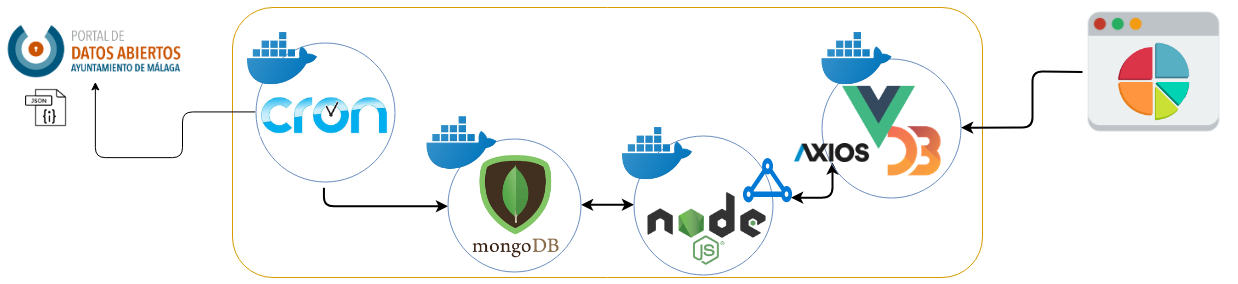
\includegraphics[width=12cm]{aireGuruArquitecture}
    \caption{Arquitecture Aire Guru}
\end{figure}

Mediante una interfaz web, muestra los datos al usuarios.\\

\begin{figure}[ht]
    \centering
    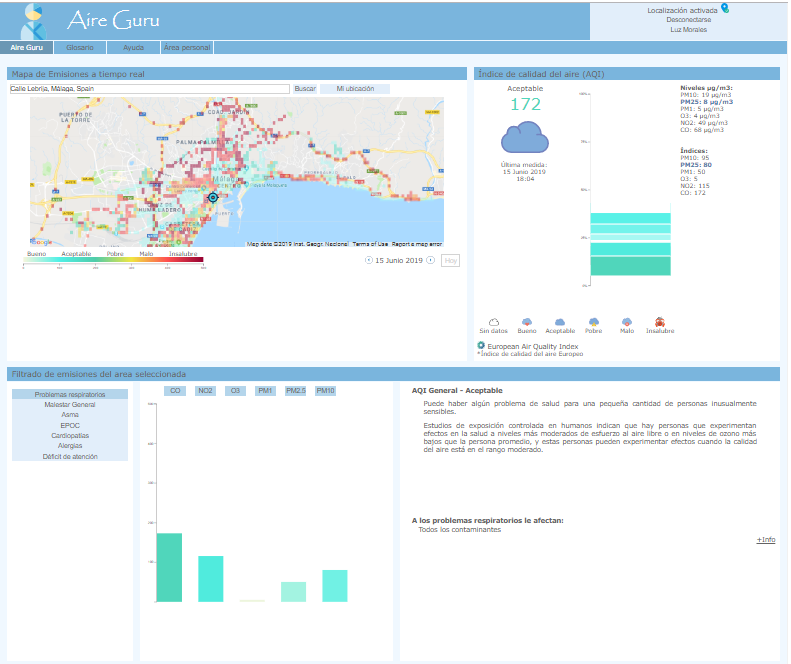
\includegraphics[width=9cm]{aireGuru}
    \caption{Aire Guru. Web Interface}
\end{figure}

Para garantizar el alcance a la mayoria de la poblacion, Aire Guru esta disponible en las direcciones webs https://www.aire.guru y https://www.airquality.guru.
Usa SSL que garantiza la encriptacion de los datos atraves de la red, ademas, cada vez mas navegadores intentan proteger a los usuarios y
solo muestran paginas que utilizar un metodo seguro. 

Como comentabamos anteriormente, todos los usuarios pueden ver la informacion basica sin necesidad de aportar ningun dato o identificarse, sin la necesidad de 
realizar ninguna descarga o instalacion y hoy en dia, casi todo el mundo esta familiarizado con la navegacion web. 
Cuando no forzamos al usuario a realizar acciones extras, como una descarga o identificacion, el usuario se sentira menos forzado a darnos una oportunidad.

\elsparagraph{Evaluation}  
\begin{itemize}
\done Los datos necesarios para nuestro modelo han sido extraidos de los datos en crudo. 
\done Infraestructura. Implementa toda la arquitectura necesaria tanto de almacenaje, procesado como visualizacion para que el usuario solo tenga que consultar 
los datos.
\done Automatiza los procesos de recoleccion de datos y los calculos necesarios para mostrar la informacion al usuario. 
\done Ofrecerles a los usuarios una pagina web libre de cargos, facilita que el usuario acceda directamente a la informacion
\end{itemize}

